\section{Result and Discussion}
\label{sec:evaluation}

%%%%%%%%%%%%%%%%%%%%%%%%%%%%%%%%%%%%%%%%%%%%%%%%%%%%%%%%%%%%%%%%%%%%
\begin{figure*}[h!]
  \centering
 
  
  \begin{subfigure}[b]{0.98\linewidth}
    \includegraphics[width=0.98\linewidth]{figs/scenes}
  \caption{Scenes}  
  \end{subfigure}
  \begin{subfigure}[b]{0.98\linewidth}
    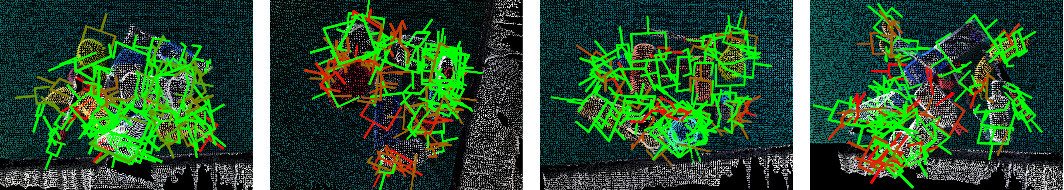
\includegraphics[width=0.98\linewidth]{figs/vg_result}
  \caption{Baseline}  
  \end{subfigure}  
  \begin{subfigure}[b]{0.98\linewidth}
    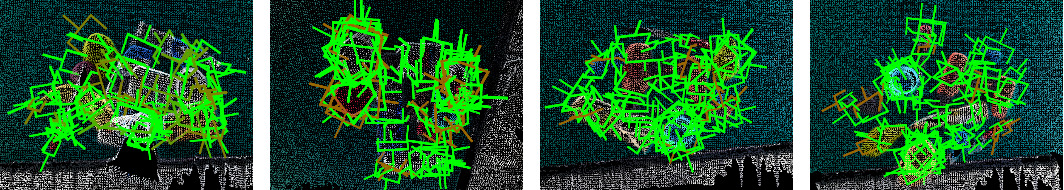
\includegraphics[width=0.98\linewidth]{figs/nvg_result}
  \caption{Ours}  
  \end{subfigure}  
    
  \caption{Examples of input scenes and predicted grasps from VoteGrasp \cite{hoang2022context} and the proposed method. The different intensity of grasp color denotes the confidence score of grasps. Green refers to the highest quality grasps and red refers to the lowest ones.}
  \label{fig:grasp_result}
\end{figure*}
%%%%%%%%%%%%%%%%%%%%%%%%%%%%%%%%%%%%%%%%%%%%%%%%%%%%%%%%%%%%%%%%%%%%

\subsection{Implementation Details}
\label{sec:implement}

%%%%%%%%%%%%%%%%%%%%%%%%%%%%%%%%%%%%%%%%%%%%%%%%%%%%%%%%%%%

\begin{table}[h]
\caption{Layer parameters of PointNet++ \cite{qi2017pointnet++} based feature learning network.}
\label{tab:layer_specs}
\begin{center}
\begin{tabular}{|l|c|c|}
\hline
layer name & input layer & layer params \\
\hline
SA1 & point cloud & (2048,0.025,[64,64,128]) \\
SA2 & SA1  & (1024,0.05,[128,128,256]) \\
SA3 & SA2 & (512,0.1,[128,128,256]) \\
SA4 & SA3 & (256,0.2,[128,128,256]) \\
FP1 & SA3, SA4 & [256,256] \\ 
FP2 & SA2, SA3 & [256,256] \\
\hline
\end{tabular}
\end{center}
\end{table}
%%%%%%%%%%%%%%%%%%%%%%%%%%%%%%%%%%%%%%%%%%%%%%%%%%%%%%%%%%%

In our implementation\footnote{Our code and other materials are available at \url{https://github.com/hoangcuongbk80/NovelVoteGrasp}}, we employ a pre-trained ResNet34 model trained on the ImageNet dataset as the encoder for RGB images. The output appearance feature from this encoder-decoder architecture comprises 256 channels. For point cloud feature extraction, we randomly sample 12,288 points from depth images and utilize a PointNet++ \cite{qi2017pointnet++}-based feature learning network, which also yields a 256-channel output. The detailed layer parameters of PointNet++ \cite{qi2017pointnet++} are displayed in Table~\ref{tab:layer_specs}. In the voting and context learning modules, we form $K=128$ clusters and produce a new feature map $\mathcal{F}_{context} \in 128 \times 512$. Subsequently, 128 grasps are generated from this new feature map. The prediction layer comprises $5 + V + 2A$ channels, with $V=120$ and $A=6$. We set $\lambda_{1}=\lambda_{2}=1.0$ and $\alpha$=$\beta$=$\gamma$=1.0. Our network is trained entirely using a batch size of 8 and optimized with Adam, employing a learning rate of 0.001 for 200 epochs. Training on a single Nvidia GeForce RTX 2080 Ti 11GB GPU takes approximately 20 hours. Regarding inference, our method requires 90ms for a single scene during the forward pass.

\subsection{Evaluation on GraspNet-1Billion}

We follow previous research \cite{fang2020graspnet} and evaluate our results on the dataset using $Precision@k$. This metric quantifies the precision of the top-k ranked grasps. To identify a predicted grasp ($G_{p}$) as a true positive, it must satisfy three conditions: (i) containing an object inside the gripper; (ii) being collision-free; (iii) exhibiting an antipodal grasp under a given friction coefficient $\mu$. The third condition is calculated based on prior works \cite{ten2017grasp, fang2020graspnet}. We denote $AP_{\mu}$ as the average $Precision@k$ for $k$ values ranging from 1 to 50, given a friction coefficient $\mu$. Additionally, we present the average of $AP_{\mu}$ across $\mu = \left\lbrace 0.2,0.4,0.6,0.8,1.0 \right\rbrace $, denoted as $AP$.


\begin{table*}[h]
\caption{The table shows the results on GraspNet-1Billion test set captured by RealSense/Kinect sensors respectively.}
\label{tab:grasp_detect_eval}
\begin{center}
\begin{tabular}{|l|c|c|c|c|c|c|c|c|c|}
\hline
& \multicolumn{3}{c|}{Seen} & \multicolumn{3}{c|}{Unseen (but similar)} & \multicolumn{3}{c|}{Novel} \\
\hline
& $AP$ & $AP_{0.8}$ & $AP_{0.4}$ & $AP$ & $AP_{0.8}$ & $AP_{0.4}$ & $AP$ & $AP_{0.8}$ & $AP_{0.4}$  \\
\hline
GG-CNN \cite{morrison2018closing} & 15.5/16.9 & 21.8/22.5 & 10.3/11.2 & 13.3/15.1 & 18.4/19.8 & 4.6/6.2 & 5.5/7.4 & 5.9/8.8 & 1.9/1.3 \\
\hline
Chu et al. \cite{chu2018real} & 16.0/17.6 & 23.7/24.7 & 10.8/12.7 & 15.4/17.4 & 20.2/21.6 & 7.1/8.9 & 7.6/8.0 & 8.7/9.3 & 2.5/1.8 \\
\hline
GPD \cite{ten2017grasp} & 22.9/24.4 & 28.5/30.2 & 12.8/13.5 & 21.3/23.2 & 27.8/28.6 & 9.6/11.3 & 8.2/9.6 & 8.9/10.1 & 2.7/3.2 \\
\hline
PointNetGPD \cite{liang2019pointnetgpd} & 26.0/27.6 & 33.0/34.2 & 15.4/17.8 & 22.7/24.4 & 29.2/30.8 & 10.8/12.8 & 9.2/10.7 & 9.9/11.2 & 2.7/3.2 \\
\hline
Fang et al. \cite{fang2020graspnet} & 27.6/29.9 & 33.4/36.2 & 17.0/19.3 & 26.1/27.8 & 34.2/33.2 & 14.2/16.6 & 10.6/11.5 & 11.3/12.9 & 4.0/3.6 \\
\hline
Gou et al. \cite{gou2021rgb} & 28.0/32.1 & 33.5/39.5 & 17.8/20.9 & 27.2/30.4 & 36.3/37.9 & 15.6/18.7 & 12.3/13.1 & 12.5/13.8 & 5.6/6.0 \\
\hline
Contact-GraspNet \cite{sundermeyer2021contact} & 29.9/31.4 & 35.2/39.0 & 19.5/21.6 & 28.2/29.0 & 37.0/35.2 & 16.3/18.9 & 13.2/13.9 & 13.5/14.7 & 6.8/7.7 \\
\hline
VoteGrasp \cite{hoang2022context}  & 34.1/37.5 & 38.9/45.6 & 24.0/27.7 & 33.0/35.9 & 40.8/43.3 & 20.5/24.7 & 16.9/18.5 & 17.0/18.5 & 10.0/10.6 \\
\hline
Ours (-VGG)  & 32.0/35.1 & 36.4/43.7 & 22.1/25.4 & 31.0/33.8 & 38.3/41.2 & 18.3/22.4 & 14.8/16.1 & 15.0/16.3 & 9.1/9.3 \\
\hline
Ours (-GGV)  & 31.4/34.6 & 35.4/42.1 & 21.4/24.2 & 30.0/32.1 & 37.4/40.0 & 17.0/21.2 & 13.5/15.8 & 14.8/15.5 & 8.3/8.8 \\
\hline
Ours & \textbf{38.5}/\textbf{39.2} & \textbf{43.1}/\textbf{46.7} & \textbf{29.3}/\textbf{30.8} & \textbf{37.2}/\textbf{38.0} & \textbf{44.1}/\textbf{45.2} & \textbf{25.1}/\textbf{28.1} & \textbf{21.5}/\textbf{21.2} & \textbf{22.5}/\textbf{22.9} & \textbf{12.6}/\textbf{13.2} \\
\hline
\end{tabular}
\end{center}
\end{table*}
%%%%%%%%%%%%%%%%%%%%%%%%%%%%%%%%%%%%%%%%%%%%%%%%%%%%%%%%%%%%%%%%%%%%

Table \ref{tab:grasp_detect_eval} and Fig. \ref{fig:grasp_result} demonstrate the performance comparison between our approach and state-of-the-art methods. The evaluation utilized the evaluation metric adopted in \cite{fang2020graspnet}, enabling a direct comparison with related works reported in \cite{fang2020graspnet, gou2021rgb}. The table showcases the evaluation outcomes categorized into "Seen," "Unseen (but similar)," and "Novel" objects, aiding in assessing the model's generalization capability. The results indicate superior performance on scenes featuring seen objects across all methods, while notably, our proposed approach consistently outperforms others, even in the challenging "Novel" category, underscoring its robust generalization capabilities.

The distinctions between "Ours (-VGG)" and "Ours (-GGV)" when compared to our complete approach ("Ours") showcase the significant impact of these modules. When excluding the VGG module, the method lacks the ability to effectively integrate RGB features, leading to a considerable reduction in performance across all evaluation categories: Seen, Unseen (but similar), and Novel objects. Similarly, without the GGV module, the model fails to appropriately fuse depth-based features, resulting in notable performance degradation in grasp detection across the board. The performance drop in both cases reaffirms the critical role played by these modules in amalgamating complementary information from RGB and depth data. It highlights their significance in capturing nuanced visual cues from different sources, which are vital for accurate and robust grasp detection. This clear decline in performance underlines the necessity of the VGG and GGV modules in our model's architecture, demonstrating their collective contribution to a more comprehensive understanding of the scene by integrating information from diverse modalities. The substantial discrepancy in results showcases that these modules are not just supplementary but rather pivotal components in leveraging the combined strengths of RGB and depth information. Their absence leads to a significant loss in the model's ability to discern crucial features necessary for precise grasp detection, emphasizing the vital role of these fusion modules in enhancing the model's performance across various object scenarios.

\textbf{Computational Time.} Our experiments were conducted on an Intel Xeon E-2716G CPU clocked at 3.7 GHz, paired with an Nvidia GeForce RTX 2080 Ti GPU featuring 11GB of memory. The runtime analysis of all evaluated methods is graphically represented in Fig. \ref{fig:runtime}. Our approach achieves a runtime of 100 ms per RGBD image. This fine balance between accuracy and speed empowers our method to proficiently generate grasp configurations in cluttered scenes, rendering it well-suited for diverse real-world scenarios.

%%%%%%%%%%%%%%%%%%%%%%%%%%%%%%%%%%%%%%%%%%%%%%%%%%%%%%%%%%%%%%%%%%%%
\begin{figure}
\centering
	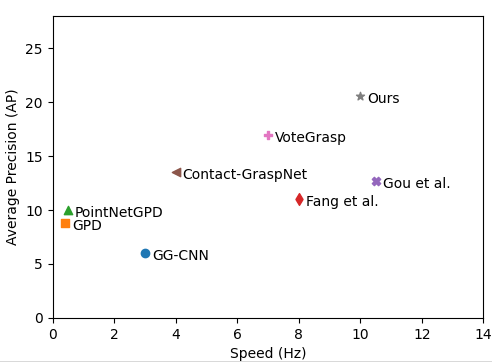
\includegraphics[width = 0.98\linewidth]{figs/time}
\caption{Comparison of running speed (Hz) and AP on GraspNet-1Billion
dataset.}
\label{fig:runtime}
\end{figure}
%%%%%%%%%%%%%%%%%%%%%%%%%%%%%%%%%%%%%%%%%%%%%%%%%%%%%%%%%%%%%%%%%%%%

\subsection{Robotic Grasping Experiment}
\label{sec:real_grasping}

The experiments were conducted with a Franka Emika Panda robot arm with 7-DOF, equipped with a parallel-jaw gripper as shown in Fig.~\ref{fig:robot1}. To capture RGBD data, we used either ASUS Xtion PRO LIVE sensor or  Microsoft Kinect sensor v2. The whole system is implemented using the ROS and MoveIt! frameworks. \\

%%%%%%%%%%%%%%%%%%%%%%%%%%%%%%%%%%%%%%%%%%%%%%%%%%%%%%%%%%%%%%%%%%%%
\begin{figure}[h!]
  \centering
 
  
  \begin{subfigure}[b]{0.98\linewidth}
    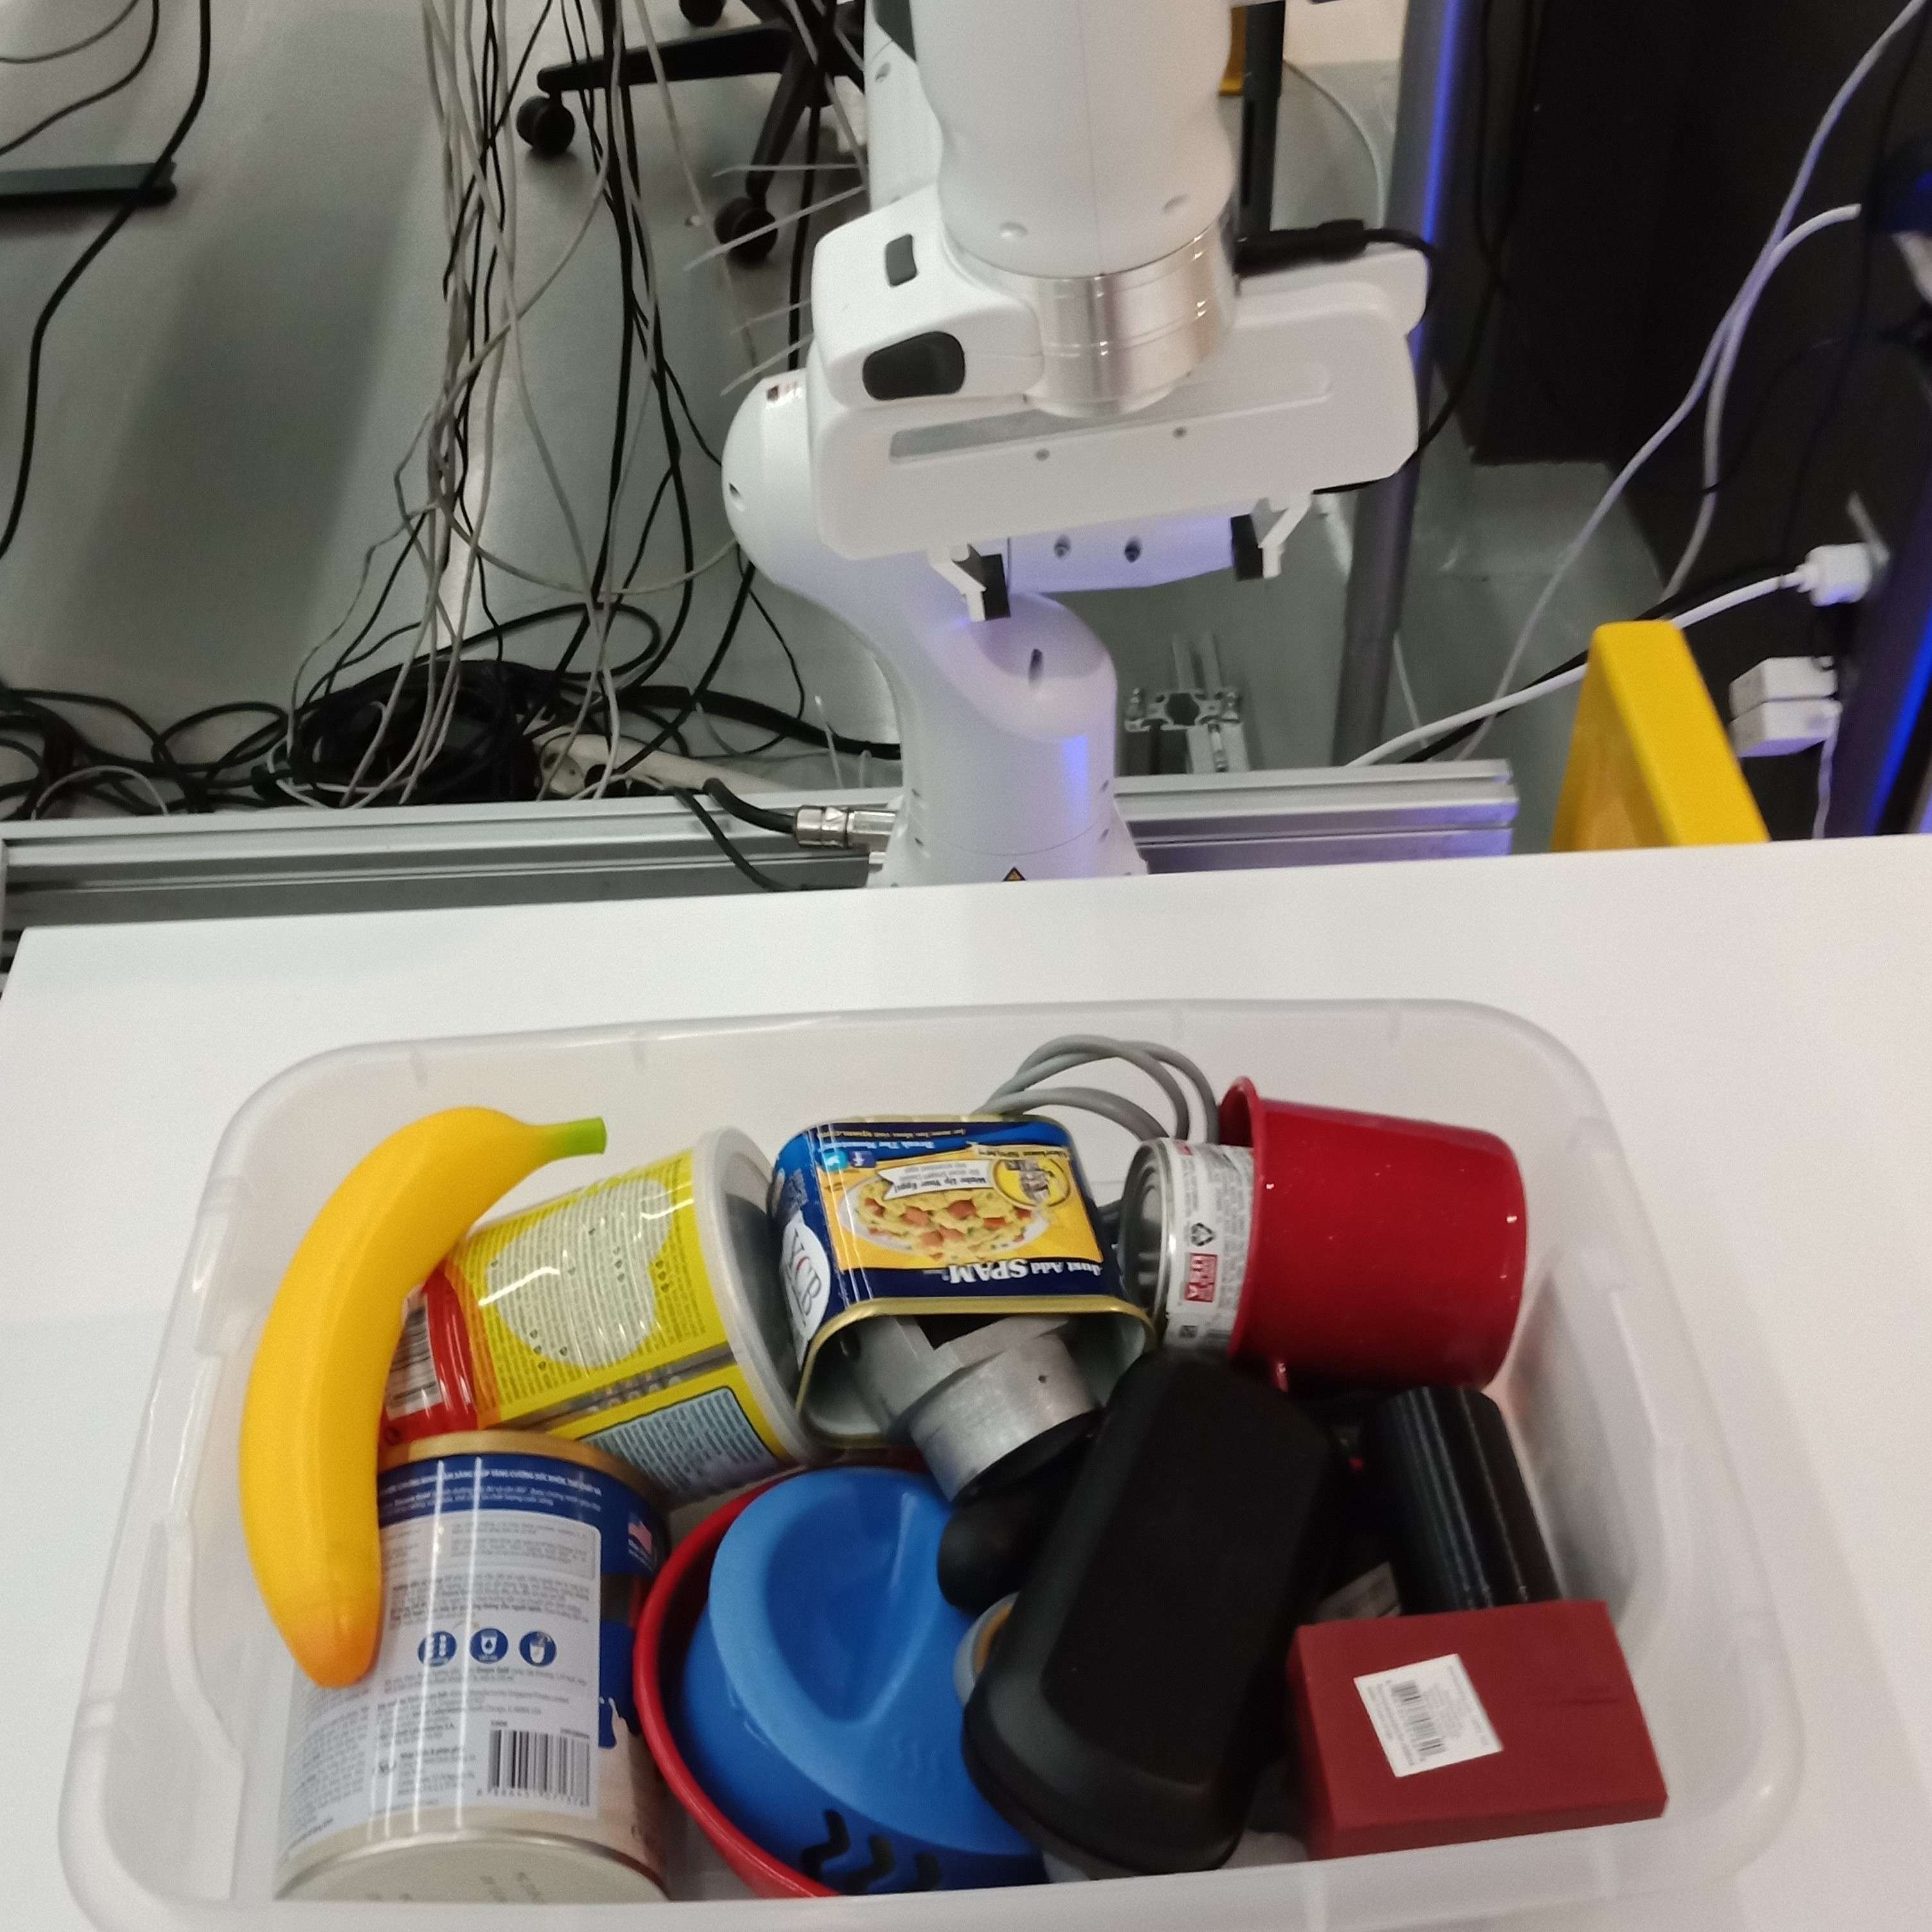
\includegraphics[width=0.48\linewidth]{figs/robot2}
    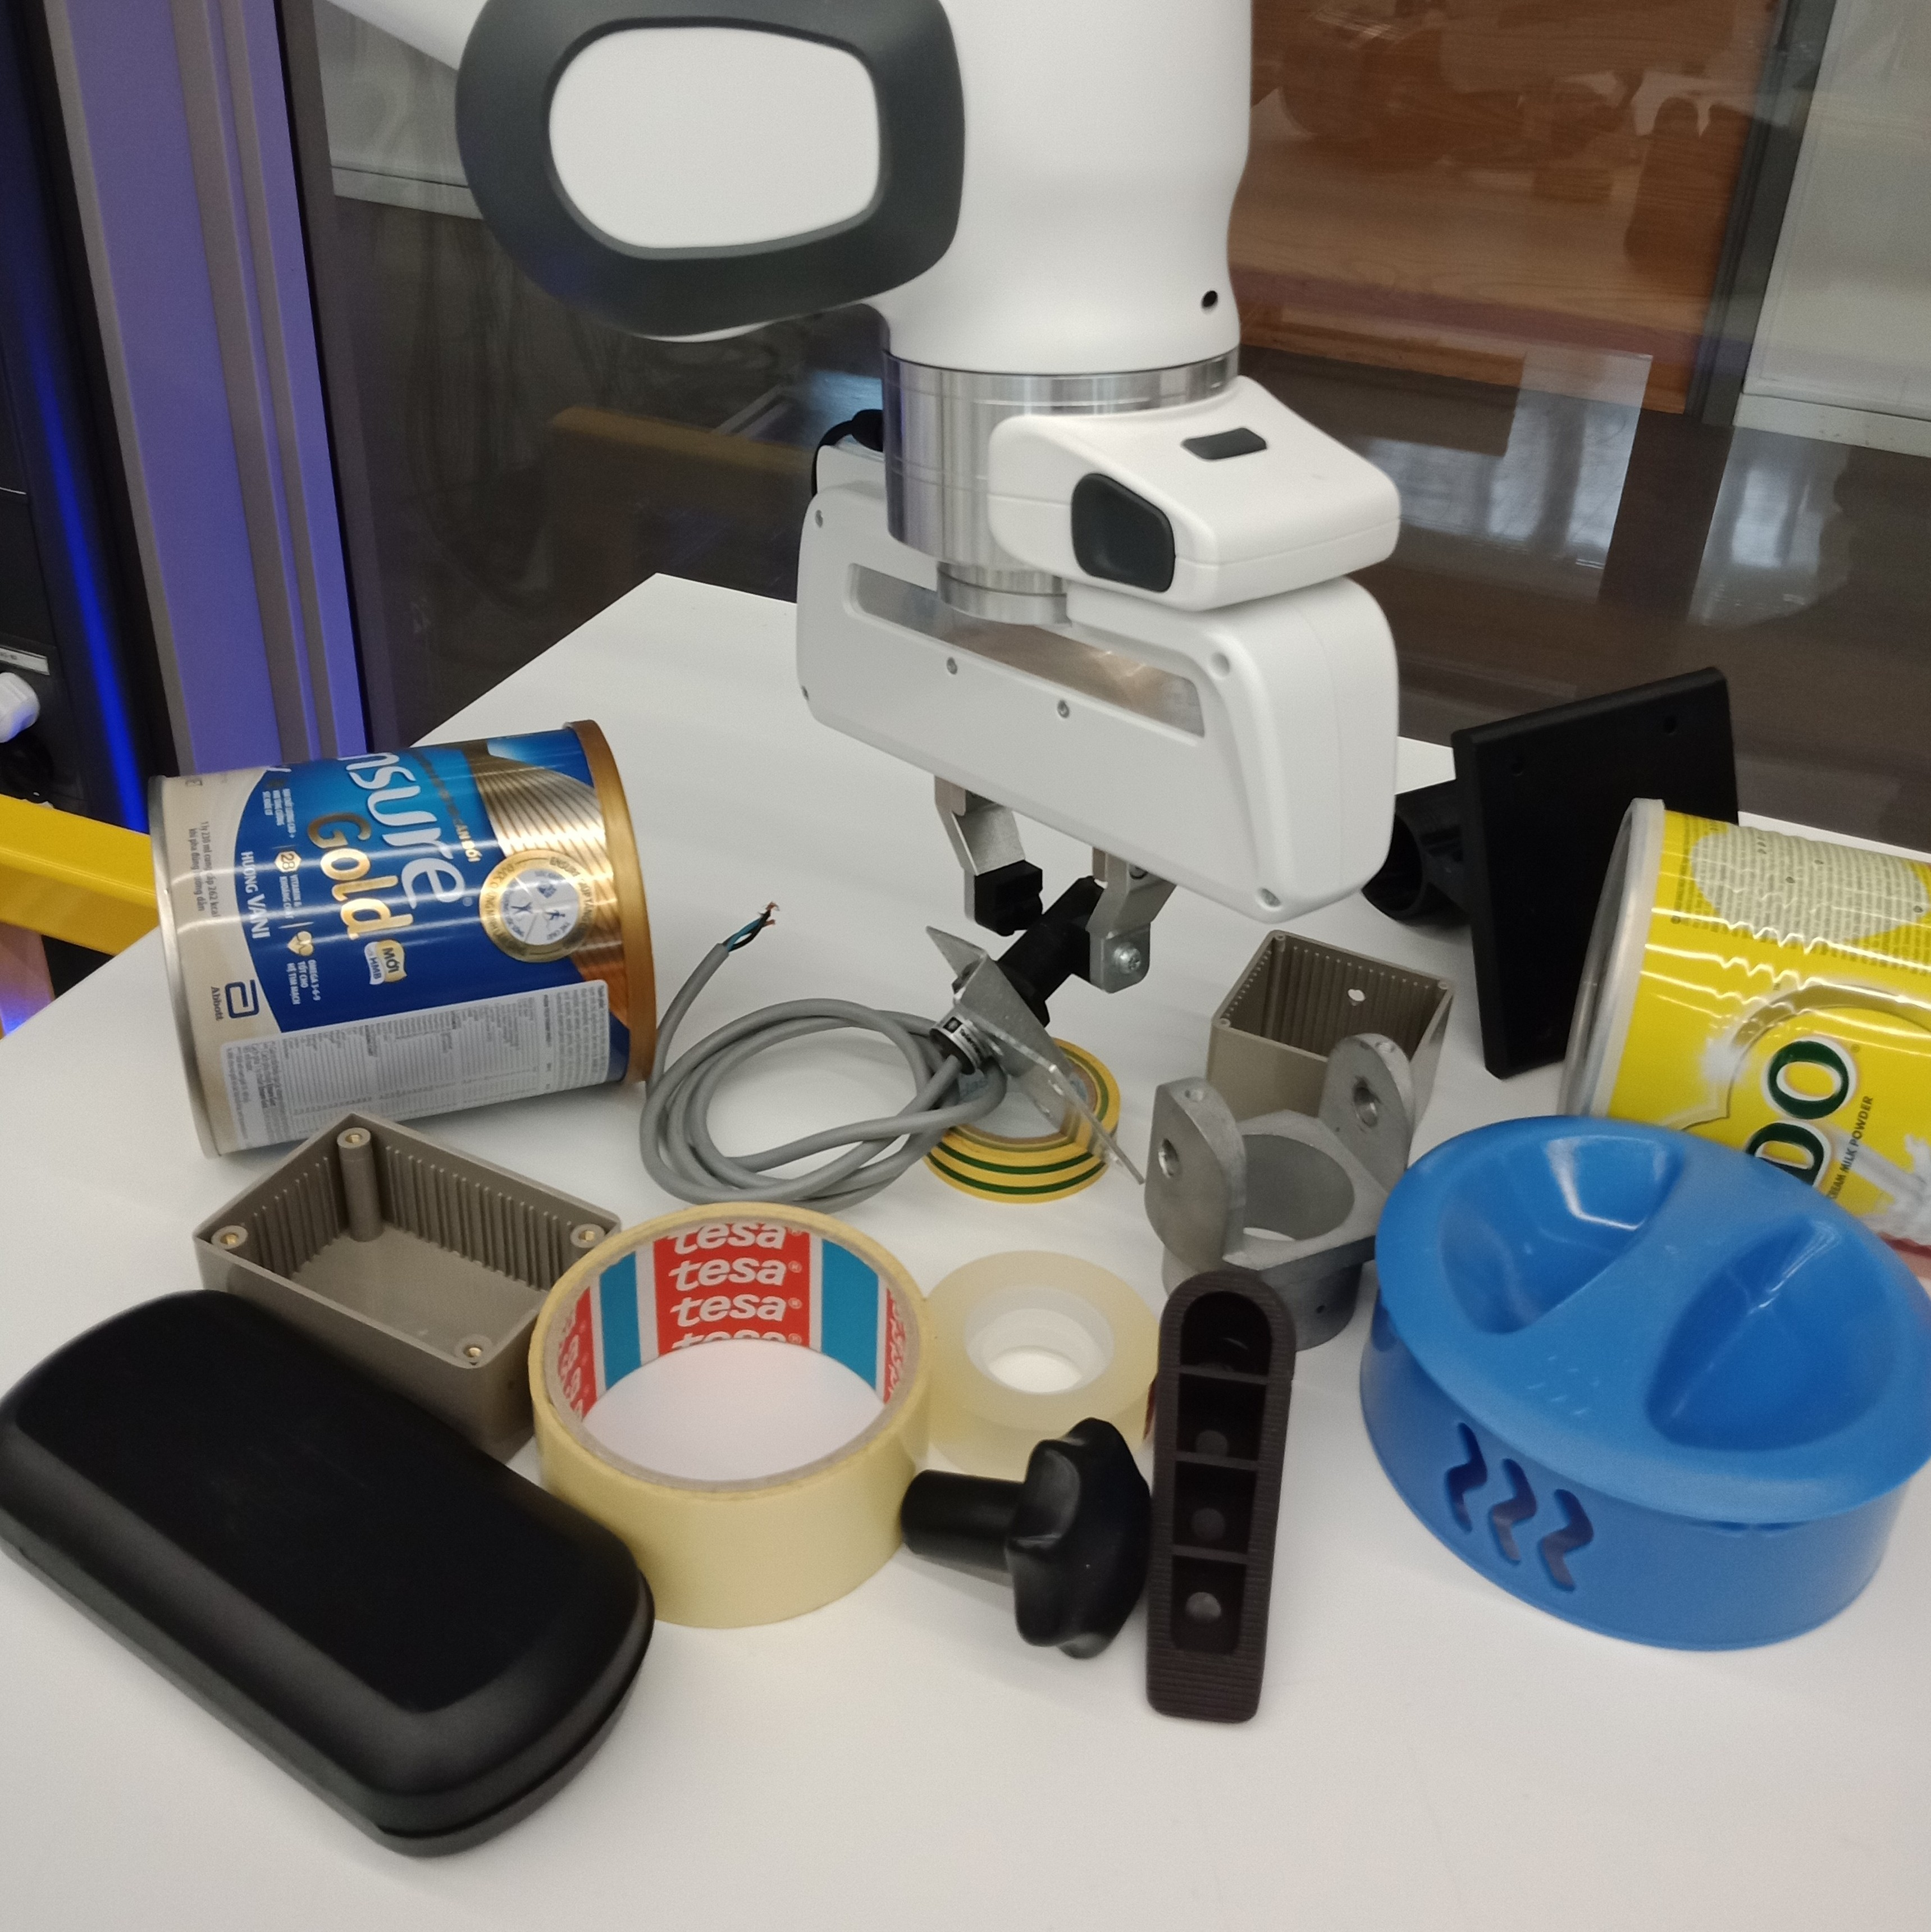
\includegraphics[width=0.48\linewidth]{figs/robot4} 
  \end{subfigure}
    
  \caption{Real-world grasping experiment.}
  \label{fig:robot1}
\end{figure}
%%%%%%%%%%%%%%%%%%%%%%%%%%%%%%%%%%%%%%%%%%%%%%%%%%%%%%%%%%%%%%%%%%%%

\begin{table}[h!]
\caption{Results of real robot experiments. The networks were trained on the GraspNet-1Billion dataset. The table shows the number of attempts, the number of successful attempts, and the grasp success rate.}
\label{tab:real_grasping}
\begin{center}
\begin{tabular}{|l|c|c|c|}
\hline
Method & Attempt & Success & Success Rate \\
\hline
GPD \cite{ten2017grasp} & 300 & 195 & 65\% \\
PointNetGPD \cite{liang2019pointnetgpd} & 300 & 201 & 67\% \\
Fang et al. \cite{fang2020graspnet} & 300 & 214 & 71\% \\
Gou et al. \cite{gou2021rgb} & 300 & 218 & 73\% \\
Contact-GraspNet \cite{sundermeyer2021contact}  & 300 & 222 & 74\% \\
VoteGrasp \cite{hoang2022context} & 300 & 234 & 78\% \\
Ours & 300 & \textbf{251} & \textbf{84}\% \\
\hline
\end{tabular}
\end{center}
\end{table}
%%%%%%%%%%%%%%%%%%%%%%%%%%%%%%%%%%%%%%%%%%%%%%%%%%%%%%%%%%%

We conducted a real-world evaluation of state-of-the-art grasp detection methods, each trained on the GraspNet-1Billion dataset for a fair comparison. GPD \cite{ten2017grasp}, PointNetGPD \cite{liang2019pointnetgpd}, and Contact-GraspNet \cite{sundermeyer2021contact} were trained using the hyperparameters specified in their respective papers. We selected novel objects tailored to fit the gripper's shapes and sizes. In each scenario, a random subset of 10-15 objects was arranged in a haphazard manner on a table, mirroring the unpredictability of real-world environments. Each method underwent 300 grasp attempts, with the robot randomly selecting objects. A grasp was deemed successful if the robot could grasp and lift the object within a single attempt. The results in Table \ref{tab:real_grasping} demonstrate our method's superiority, achieving an 84\% success rate outperforming all other methods. This highlights the proposed framework's efficacy in real-world grasping scenarios, attributing the increased success rate to the integration of estimated depth data, underscoring the significance of richer input data for precise and effective.  \\

\section{Conclusions}

In this study, we addressed the fundamental challenge of grasp generation in robotic manipulation by introducing an innovative approach that bypasses the need for specialized depth sensors. Our method revolutionizes grasp generation by leveraging tailored deep learning techniques to estimate depth from color (RGB) images directly. This paradigm shift allows the computation of predicted point clouds solely from RGB inputs, eliminating the dependency on traditional depth sensors. A pivotal contribution lies in the development of a fusion module adept at seamlessly integrating features derived from RGB images with those inferred from predicted point clouds. This fusion process harnesses the strengths of both modalities, significantly enhancing grasp configurations. Experimental evaluations unequivocally validate the effectiveness of our approach, demonstrating its superiority in generating grasp configurations compared to existing methods. Future endeavors in these outlined directions hold the promise of further enhancing the versatility, adaptability, and real-world applicability of grasp generation in robotics.